\chapter[Latent Score-based Data Assimilation]{Latent Score-based\\Data Assimilation} \label{chap:appa}

\begin{quote}
    \textit{Imagine a system on a rotating sphere that is 8000 miles wide, consists of different materials, different gases that have different properties (one of the most important of which, water, exists in different concentrations), heated by a nuclear reactor 98 million miles away. Then, just to make life interesting, this sphere is oriented such that, as it revolves around the nuclear reactor, it is heated differently at different locations at different times of the year. Then, someone is asked to watch the mixture of gases, a fluid only 20 miles deep, that covers an area of 250 million square miles, and to predict the state of that fluid at one point on the sphere two days from now. This is the problem weather forecasters face.}

    \begin{flushright}
        --- Robert T. Ryan (1982) \nocite{ryan1982weather}
    \end{flushright}
\end{quote}

\vspace{2em}

\begin{addendum}{\Large\scshape Addendum}

This chapter appeared previously as

\begin{itemize}[leftmargin=1em]
    \item[] \fullcite{andry2025appa}.
\end{itemize}

Gérôme and Sacha implemented the methods, conducted the experiments, interpreted the results, and wrote most of the manuscript. François came up with the methods, supervised the codebase, and wrote the technical parts of the manuscript. Omer, Victor and Matthias contributed to the codebase and the visualization of the results. Elise provided valuable domain knowledge. Gilles supervised the project, suggested experiments, and participated in the writing.

For the version presented in this chapter, we have edited the structure and content of the manuscript to be consistent with the rest of this document. At the time of writing, the Appa project is still in progress and is not published within a peer-reviewed venue. Nevertheless, we wish to include this early version in this dissertation, as it is a logical continuation of our work.

\end{addendum}

\section*{Abstract}

While deep learning has been transformative for numerical weather prediction, the assimilation step preceding forecasting that estimates the current atmospheric state from observational data remains challenging. In this work, we introduce Appa, a score-based data assimilation model generating global atmospheric trajectories at \qty{0.25}{\degree} resolution and 1-hour intervals. Powered by a 565M latent diffusion model trained on ERA5, Appa can be conditioned on arbitrary observations to infer plausible trajectories, without retraining. Our probabilistic framework handles reanalysis, filtering, and forecasting as special cases. Results establish latent score-based data assimilation as a promising foundation for future global atmospheric modeling systems.

\section{Introduction} \label{sec:appa-introduction}

Data assimilation combines observational data with physical models to estimate atmospheric states. Formally, let $x^{1:L} = (x^1, x^2, \dots, x^L) \in \mathbb{R}^{L \times V \times C}$ denote a trajectory of $L$ atmospheric states, each represented as $C$ physical fields over a mesh of $V$ vertices. Let $p(x^1)$ be the initial state prior and $p(x^{i+1} \mid x^i)$ the transition dynamics. Observations $y^{1:L} \in \mathbb{R}^{M_1 + \dots + M_L}$ of the states $x^{1:L}$ follow an observation process $p(y^i \mid x^i)$, generally formulated as $y^i = \mathcal{H}^i(x^i) + \eta^i$, where the measurement functions $\mathcal{H}^i: \mathbb{R}^{V \times C} \mapsto \mathbb{R}^{M_i}$ can be non-linear and $\eta^i \in \mathbb{R}^{M_i}$ represents observational error that accounts for instrumental noise and systematic uncertainties. The goal of data assimilation is to infer plausible trajectories $x^{1:L}$ consistent with the observations $y^{1:L}$, that is, to estimate the trajectory posterior
\begin{equation} \label{eq:general-assim}
    p(x^{1:L} \mid y^{1:L}) \propto p(x^1) \prod_{i=1}^{L-1} p(x^{i+1} \mid x^i) \prod_{i=1}^{L} p(y^i \mid x^i) \, .
\end{equation}
While Eq.~\eqref{eq:general-assim} defines the general assimilation problem, assimilation tasks correspond to specific choices of states $x^i$ to infer and observations $y^i$ to take into account. In this work, we focus on three special cases:
\begin{align}
    \textbf{Reanalysis}  \quad & p(x^{1:L} \mid y^{1:L}) \, , \label{eq:reanalysis} \\
    \textbf{Filtering}   \quad & p(x^L \mid y^{1:L}) \, , \label{eq:filtering} \\
    \textbf{Forecasting} \quad & p(x^{K+1:L} \mid y^{1:K}) \, . \label{eq:forecast}
\end{align}
Reanalysis aims to reconstruct full trajectories from historical observations. The primary purpose of reanalysis is to create datasets of historical data for the land, atmosphere, and oceans. These datasets enable scientists to better monitor and understand the climate, conduct surveys, and develop new weather models. Filtering, in contrast, only infers the posterior distribution of the last/current state $x^L$. This step is crucial to initialize global weather models in numerical weather prediction. Forecasting, as its name suggests, extends beyond the observed segment, producing posterior distributions over future states. The forecasting problem is often decomposed into first estimating the current state $x^K$ from $y^{1:K}$, and then predicting its evolution.

Traditional assimilation methods like 4D-Var~\cite{lorenc1986analysis, ledimet1986variational, tremolet2006accounting, tremolet2007modelerror, fisher2011weakconstraint} or ensemble Kalman filters~\cite{evensen1994sequential, bishop2001adaptive, anderson2007adaptive, hunt2007efficient, evensen2009data} are effective but rely on linearization and differentiation of the transition dynamics, which is very expensive at a global scale. In addition, 4D-Var provides point estimates instead of a posterior distribution~\cite{carrassi2018data}. Recent data-driven approaches~\cite{cheng2023machine, huang2024diffda, xu2025fuxida, fablet2021joint, andrychowicz2023deep} integrate deep learning into assimilation, but suffer from limited resolution, lack of uncertainty quantification, and require retraining for new observation configurations.

\section{Appa} \label{sec:appa}

Appa combines score-based data assimilation~\cite{rozet2023scorebased, rozet2023scorebaseda, schmidt2025generative} with latent diffusion-based physics emulation~\cite{rozet2025lost}, scaled to the global atmospheric system at \qty{0.25}{\degree} resolution and 1-hour intervals. It consists of (1) a 340M encoder-decoder pair $(E_\psi, D_\psi)$ that compresses atmospheric states $x^i$ into $530\times$ smaller latent representations $z^i \sim \mathcal{N}(z^i \mid E_\psi(x^i), \sigma_z^2 I)$ and (2) a 225M diffusion transformer (DiT) \cite{peebles2023scalable} that generates windows $z^{i:i+W}$ of $W = 24$ consecutive latent states.

The encoder and decoder are trained to minimize the $L_2$ error between states $x^i$ and their reconstruction $\hat{x}^i = D_\psi(z^i)$. The DiT $d_\phi(z^{i:i+W}_t)$ is trained to estimate the denoising posterior mean $\mathbb{E}[z^{i:i+W} \mid z^{i:i+W}_t]$ for noisy latent states $z^{i:i+W}_t \sim \mathcal{N}(\alpha_t \, z^{i:i+W}, \sigma_t^2 I)$. Tweedie's formula~\cite{tweedie1947functions, efron2011tweedies, kim2021noise2score}
\begin{equation}
    \mathbb{E} \big[z^{i:i+W} \mid z^{i:i+W}_t\big] = \frac{z^{i:i+W}_t + \sigma^2_t \, \grad{z^{i:i+W}_t} \log p(z^{i:i+W}_t)}{\alpha_t}
\end{equation}
then gives access to the prior score $\grad{z^{i:i+W}_t} \log p(z^{i:i+W}_t)$ necessary to simulate the reverse diffusion process \cite{song2021scorebased}. As in the SDA~\cite{rozet2023scorebased, rozet2023scorebaseda} framework, the score over longer trajectories $z^{1:L}_t$ is approximated by composing the scores over windows $z^{i:i+W}_t$. Algorithm \ref{alg:appa-composing} generalizes SDA's composition algorithm by introducing a time stride $\Delta \geq 1$ between consecutive windows. Using a larger stride reduces the window overlap and, therefore, the number of network evaluations.

\begin{figure}[b]
\begin{minipage}[t]{0.49\textwidth}%
\vspace{-1em}
\begin{algorithm}[H]
    \caption{Training $d_\phi(z^{i:i+W}_t)$} \label{alg:appa-training}
    \begin{algorithmic}[1]
        \For{$n = 1$ to $N$}
            \State $x^{1:L} \sim p(x^{1:L})$
            \State $i \sim \mathcal{U}(\{1, \dots, L-W\})$
            \State $t \sim \mathcal{U}(0, 1) \, , \varepsilon \sim \mathcal{N}(0, I)$
            \For{$j = i$ to $i + W$}
                \State $z_j \gets E_\psi(x_j)$
            \EndFor{}
            \State $z^{i:i+W}_t \gets \alpha_t \, z^{i:i+W} + \sigma_t \, \varepsilon$
            \State $\displaystyle \ell \gets \big\| d_\phi(z^{i:i+W}_t) - z^{i:i+W} \big\|^2_2$
            \State $\phi \gets \Call{SGD}{\phi, \grad{\phi} \, \ell}$
        \EndFor{}
	\end{algorithmic}
\end{algorithm}
\end{minipage}%
\hfill%
\begin{minipage}[t]{0.49\textwidth}%
\vspace{-1em}
\begin{algorithm}[H]
    \caption{Composing $d_\phi(z^{i:i+W}_t)$} \label{alg:appa-composing}
    \begin{algorithmic}[1]
        \Function{$d_\phi(z^{1:L}_t)$}{}
            \State $a \gets \nicefrac{(W - \Delta)}{2}$
            \State $b \gets a + \Delta$
            \State $E_{1:a} \gets d_\phi(z^{1:1+W}_t)[:\!a]$
            \For{$n = 0$ to $\nicefrac{(L - W)}{\Delta} + 1$}
                \State $i \gets 1 + n \Delta$
                \State $E_{i+a:i+b} \gets d_\phi(z^{i:i+W}_t)[a\!:\!b]$
            \EndFor{}
            \State $E_{L-W+b:L} \gets d_\phi(z^{L-W:L}_t)[b\!:]$
            \State \Return{$E_{1:L}$}
        \EndFunction{}
	\end{algorithmic}
\end{algorithm}
\end{minipage}
\end{figure}

\paragraph{Sampling conditionally on observations}
To sample from the posterior $p(z^{1:L} \mid y^{1:L})$, we replace the prior score in the reverse diffusion process with the posterior score
\begin{equation} \label{eq:score-bayes}
    \grad{z^{1:L}_t} \log p(z^{1:L}_t \mid y^{1:L}) = \grad{z^{1:L}_t} \log p(z^{1:L}_t) + \grad{z^{1:L}_t} \log p(y^{1:L} \mid z^{1:L}_t) \, .
\end{equation}
The prior score $\grad{z^{1:L}_t} \log p(z^{1:L}_t)$ is obtained with the denoiser $d_\phi(z^{i:i+W}_t)$ and Algorithm \ref{alg:appa-composing}, while the likelihood score $\grad{z^{1:L}_t} \log p(y^{1:L} \mid z^{1:L}_t)$ can be approximated \cite{chung2023diffusion, rozet2023scorebased, rozet2024learning, daras2024survey} without retraining under moderate assumptions on the observation process $p(y^i \mid x^i)$.

The key challenge is that the observation process $p(y^i \mid x^i)$ is defined in terms of atmospheric state $x^i$ rather than latent state $z^i$. To address this issue, we approximate the mapping from $z^i$ to $y^i$ as the composition of the decoder $D_\psi$ and measurement function $\mathcal{H}^i$. Formally, we assume
\begin{equation}
    p(y^{1:L} \mid z^{1:L}) \approx \mathcal{N} \left( y^{1:L} \mid \mathcal{A}(z^{1:L}), \Sigma_{y} \right)
\end{equation}
such that $\mathcal{A}(z^{1:L}) = \big( \mathcal{H}^{1}(D_\psi(z^{1})) \dots \mathcal{H}^{L}(D_\psi(z^{L})) \big)$ and $\Sigma_y$ is the covariance of $\eta^{1:L}$. With this formulation, off-the-shelf posterior sampling algorithms~\cite{daras2024survey} can be used to infer atmospheric trajectories conditionally on observational data. In this work, we adapt moment matching posterior sampling (MMPS) \cite{rozet2024learning} to non-linear measurement functions $\mathcal{A}$ by estimating the covariance with the Jacobian $A$ of $\mathcal{A}$, yielding the following perturbed likelihood approximation
\begin{equation}
    p(y^{1:L} \mid z^{1:L}_t) \approx \mathcal{N} \left(y^{1:L} \mid \mathcal{A} \big( \mathbb{E} \big[z^{1:L} \mid z^{1:L}_t\big] \big), \Sigma_y + A \, \mathbb{V} \big[z^{1:L} \mid z^{1:L}_t\big] \, A^\top \right) \, .
\end{equation}
Once the posterior score $\grad{z^{1:L}_t} \log p(z^{1:L}_t \mid y^{1:L})$ is available, we simulate the reverse diffusion process \cite{song2021scorebased} to sample from $p(z^{1:L} \mid y^{1:L})$. Afterwards, the latent trajectories $z^{1:L}$ are mapped back to the atmospheric space via the decoder $\hat{x}^i = D_\psi(z^i)$.

\section{Experiments} \label{sec:appa-experiments}

We train and evaluate Appa on the ERA5 reanalysis dataset \cite{hersbach2020era5}. We follow standard chronological splitting for evaluation: 1993--2019 for training, 2020 for validation, and 2021--2023 for testing. We consider 6 surface and 5 atmospheric fields across 13 pressure levels for a total of $C=71$ physical fields. In the following, we evaluate the latent representation quality, performance across assimilation tasks, and compare against existing assimilation and forecasting methods.

\paragraph{Latent representation}
Despite the large ($530 \times$) compression factor, standardized reconstruction root-mean-squared error (RMSE) is mostly below 0.1, with slightly higher values for humidity and winds, and lower ones for surface and low-altitude fields, as shown in Figure~\ref{fig:ae-rmse}. Power spectra of state reconstructions match the ground-truth closely at large scales, but slightly diverge for wavelengths smaller than \qty{100}{\kilo\meter}, which is expected behavior from $L_2$ driven compression \cite{rozet2024learning}. Since atmospheric energy concentrates at larger scales, the majority of energy is preserved. Overall, our autoencoder attains similar or better performance than prior neural compression methods of ERA5 \cite{mirowski2024neural}.

\begin{figure}[!b]
    \vspace{-0.5em}
    \centering
    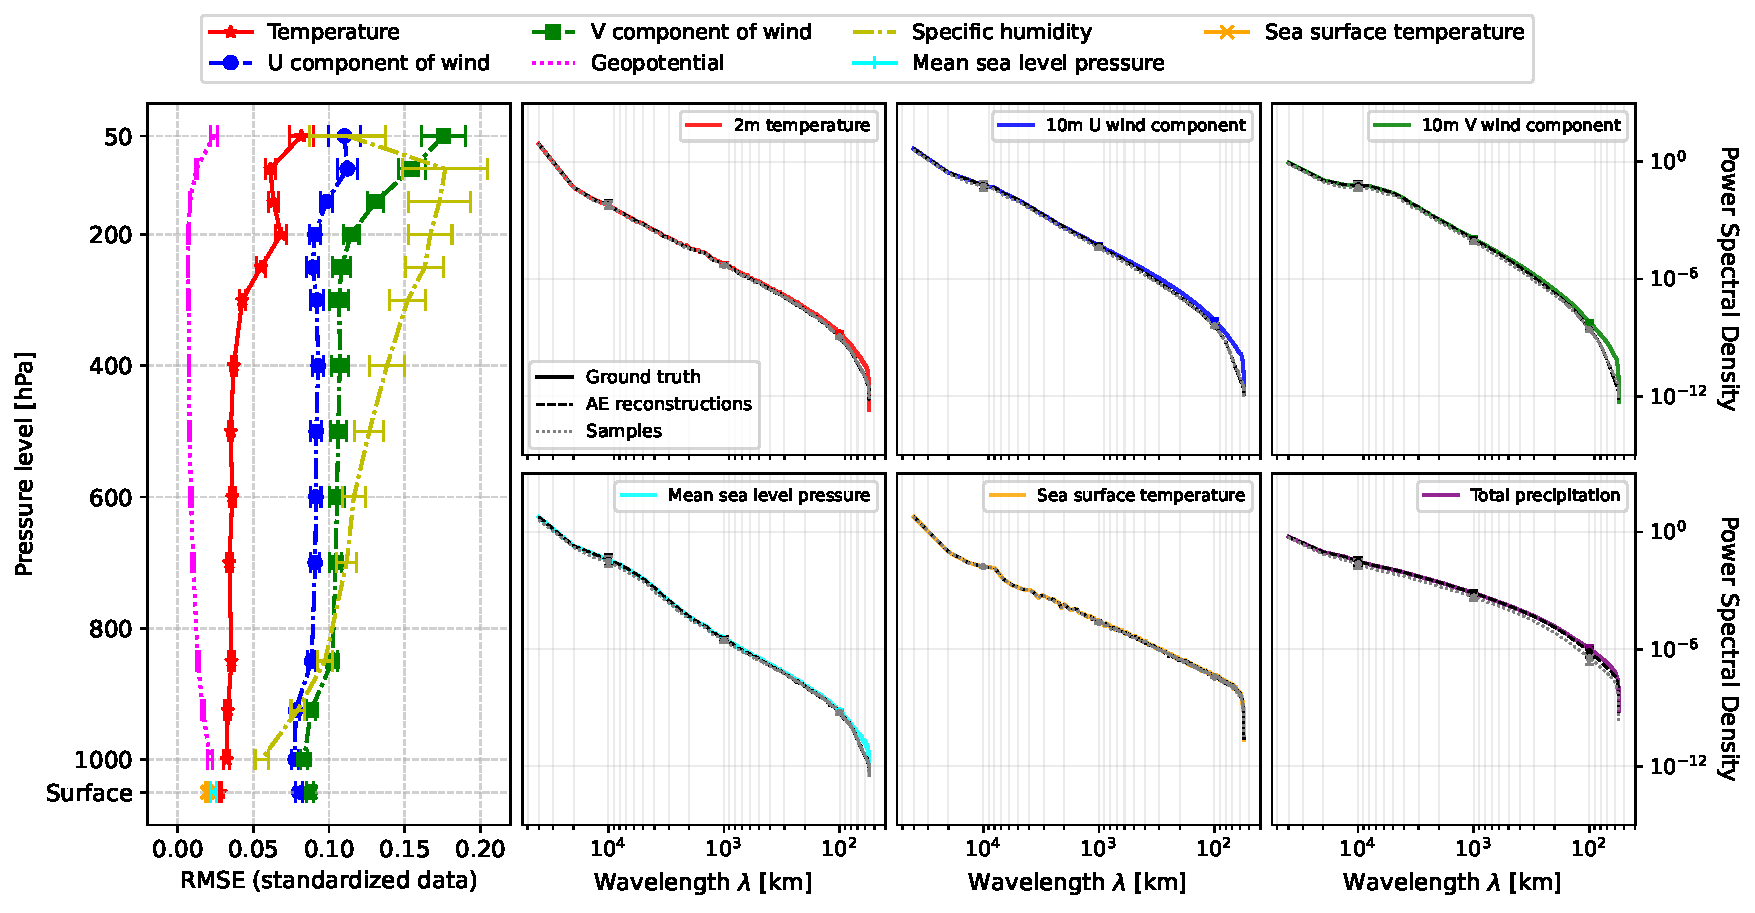
\includegraphics[width=\textwidth]{./chapters/appa/figures/ae_rmse_spectra.pdf}
    \caption{Standardized autoencoder reconstruction RMSE (left) and power spectra of Appa's prior samples (right) between January and December 2021. Lower-frequency fields (temperature, geopotential) are reconstructed more accurately than volatile fields (humidity, wind). Near-surface fields benefit from altitude-weighting. Power spectral density shows close alignment across wavelenghts, with deviations below \qty{100}{\kilo\meter}.}
    \label{fig:ae-rmse}
\end{figure}

\paragraph{Assimilation}
We evaluate Appa across four tasks: reanalysis, filtering, observational forecasting, and full-state forecasting. For the first three tasks, we assimilate synthetic ground station observations of all surface fields and simulated satellite scans of the 5 atmospheric fields. The station network consists of \num{11000} real-world measurement locations~\cite{noaanationalcentersofenvironmentalinformation1999global} covering roughly $\qty{1}{\percent}$ of \qty{0.25}{\degree} grid points. Ground stations are sparse and globally distributed, while satellite orbital paths provide dense coverage within a limited spatio-temporal domain. Observations are modeled as Gaussian distributions centered on the ERA5 ground-truth, with noise levels of $\qty{1}{\percent}$ for ground stations and $\qty{10}{\percent}$ for satellites, relative to the observed field's respective standard deviation. Each assimilation is carried with 10 ensemble members.

Figure~\ref{fig:reanalysis-quant} summarizes Appa's quantitative performance. Further results can be found in Appendix \ref{app:appa-additional-results}. For reanalysis and filtering, conditioning on longer assimilation windows improves both skill and CRPS but gains saturate beyond 24 hours. Forecasting's skill decays gradually with lead time but remains significantly stronger than the persistence baseline. Observational forecasts, conditioned on the last 12 hours of a day-long assimilation, start at skill and CRPS levels comparable to the reanalysis plateau. Full-state forecasts, initialized from two complete states, start with lower errors but eventually converge to similar performance. The error growth lies between two baselines: steeper than IFS~\cite{ecmwf2020ifs} but parallel to GraphDOP~\cite{alexe2024graphdop}. This suggests that the learned latent representation does not introduce artifacts that strongly impede the learning of the dynamics, supporting \textcite{rozet2025lost}'s findings.

\begin{figure}[!h]
    \centering
    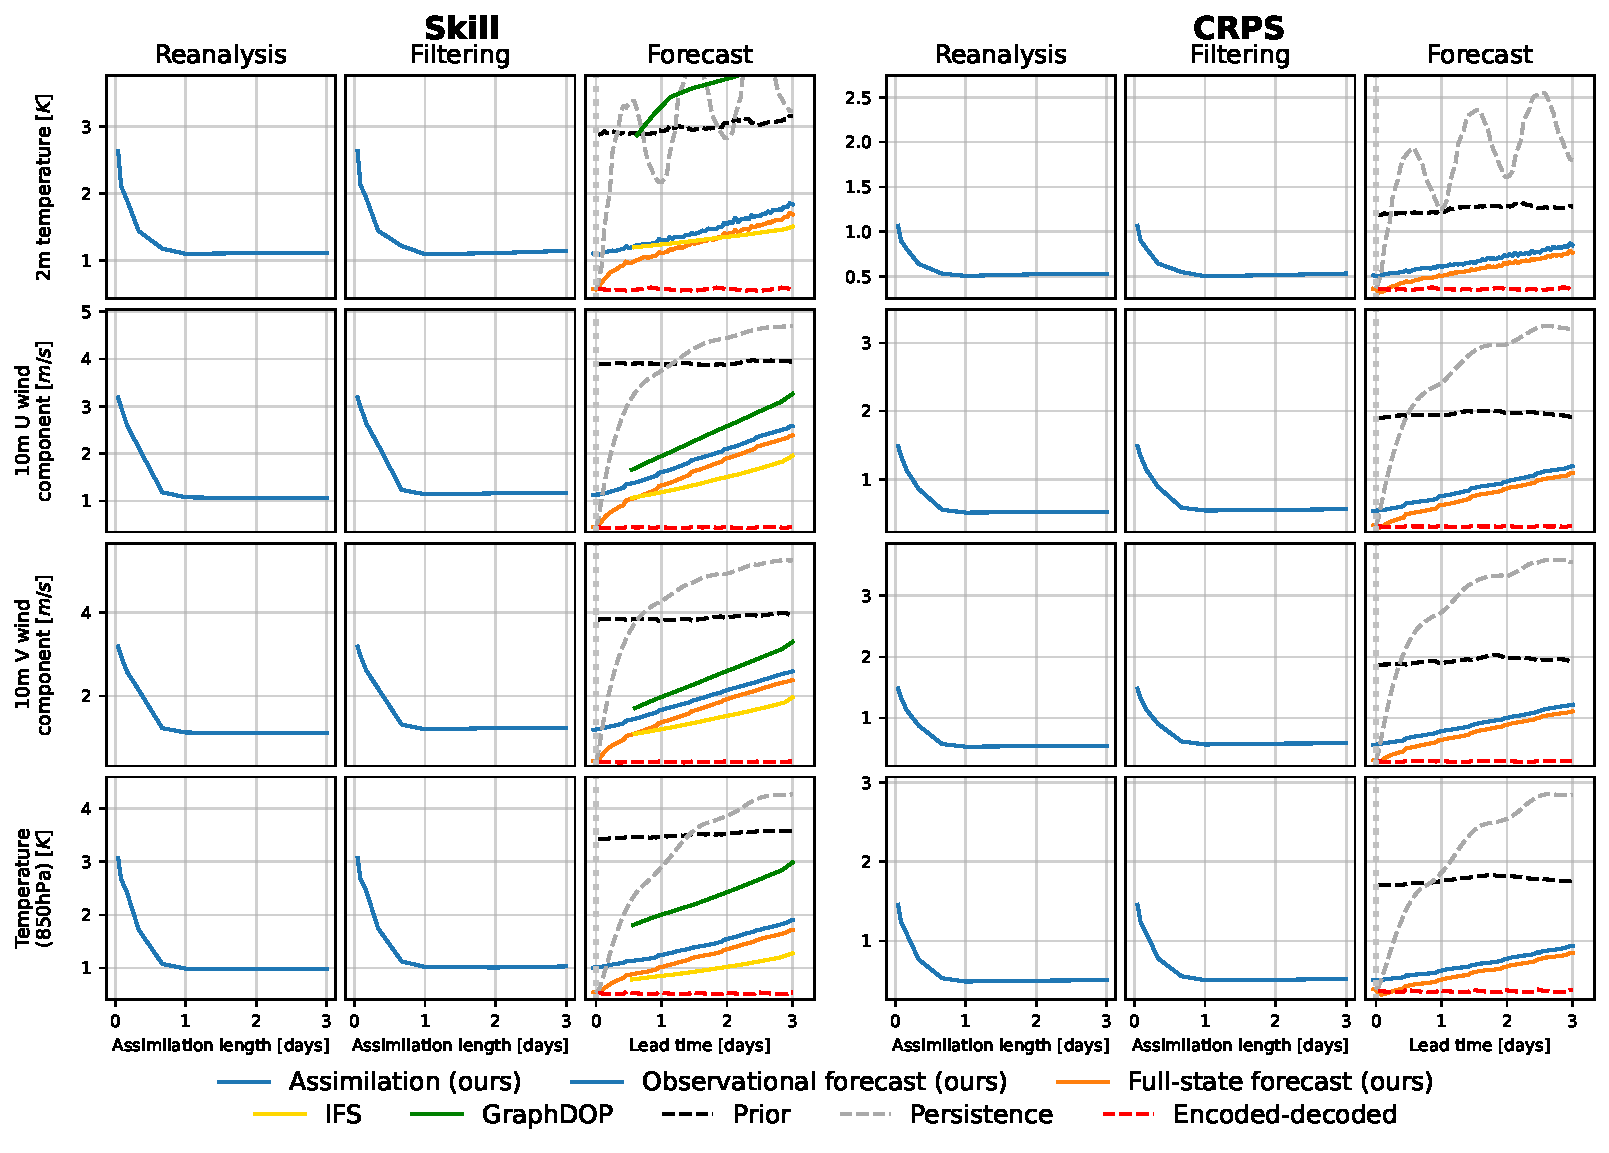
\includegraphics[width=\textwidth]{./chapters/appa/figures/skill_crps_main_2023.pdf}
    \caption{Skill and continuous ranked probability score (CRPS) of representative fields in assimilation tasks over January 2023. Reanalysis metrics are averaged over assimilation windows $x^{1:L}$, while filtering only considers the last assimilated state $x^L$. Both improve with longer assimilation windows, but eventually stagnate. Forecasts gradually lose skill over lead time. IFS~\cite{ecmwf2020ifs} and GraphDOP~\cite{alexe2024graphdop} are reported for reference.}
    \label{fig:reanalysis-quant}
\end{figure}

\section{Discussion} \label{sec:appa-discussion}

\paragraph{Summary}
We introduce Appa, a latent score-based data assimilation model that produces global atmospheric trajectories efficiently by operating in a compressed latent space. Appa can be conditioned on arbitrary observations without retraining, providing access to the full posterior distribution of consistent trajectories. Our results demonstrate that Appa flexibly handles reanalysis, filtering, and forecasting within a unified probabilistic framework, while remaining competitive with baselines.

\paragraph{Limitations and future work}
While Appa demonstrates strong assimilation and forecasting capabilities, it remains a proof of concept that isn't ready yet for operational applications. We foresee several possible improvements. First, we should move from simplified synthetic observations to realistic measurements, such as satellite radiances. Improving physical consistency is also critical, especially for forecasting tasks where Appa falls short of standard baselines such as IFS~\cite{ecmwf2020ifs}. Replacing guidance-based posterior sampling with explicit conditioning on past states, as in GenCast~\cite{price2025probabilistic} and LoLA~\cite{rozet2024learning}, could improve both accuracy and efficiency of forecasting. In terms of statistical assessment, the calibration of posterior distributions deserves further validation. The approximations present in our method, notably while estimating the prior and likelihood scores, introduce errors which are hard to quantify without proper statistical validation. Computational efficiency of reanalysis remains a challenge as well, as conditioning with respect to atmospheric observations requires decoding latent states repeatedly. Projecting observations into latent space could mitigate this bottleneck \cite{raphaeli2025silo}. Finally, our comparison to other models is still preliminary due to the discrepancies in experimental configurations. Fair evaluation against IFS~\cite{ecmwf2020ifs}, GraphDOP~\cite{alexe2024graphdop} and other models \cite{lam2023learning, price2025probabilistic} would help position Appa within the spectrum of global atmospheric models.

\section*{Acknowledgments}

Gérôme Andry, François Rozet, Sacha Lewin, and Elise Faulx are research fellows of the F.R.S.-FNRS (Belgium) and acknowledge its financial support. Omer Rochman acknowledges the financial support of the Walloon Region under grant no. 2.0102.35 (ARIAC by Digital Wallonia 4.AI). Victor Mangeleer is a research fellow part of the Multiple THreats on Ocean health (MiTHO) project and acknowledges funding from the European Space Agency (ESA).

The present research benefited from computational resources made available on Lucia, the Tier-1 supercomputer of the Walloon Region, infrastructure funded by the Walloon Region under the grant no. 1910247. The computational resources have been provided by the Consortium des Équipements de Calcul Intensif (CÉCI), funded by the Fonds de la Recherche Scientifique de Belgique (F.R.S.-FNRS) under the grant no. 2.5020.11 and by the Walloon Region.

\clearpage
\section*{References}

\printbibliography[heading=none]

\begin{subappendices}

\clearpage
\section{Data} \label{app:appa-data}

ERA5 is a global deterministic reanalysis dataset from ECMWF that provides high-resolution (\qty{0.25}{\degree}) hourly estimates of atmospheric, land, and oceanic fields from 1959 onward~\cite{hersbach2020era5}. It assimilates observations into a numerical weather prediction model using 4D-Var data assimilation.

In this work, we use a subset of ERA5 data, defined on a \qty{0.25}{\degree} equiangular grid with 13 pressure levels: 50, 100, 150, 200, 250, 300, 400, 500, 600, 700, 850, 925, and 1000 \unit{\hecto\pascal}. Following \textcite{lam2023learning}, we restrict the temporal coverage of the dataset to the 1993--2021 period, with data split into training (1993--2019), validation (2020), and testing (2021--2023). ERA5 data was downloaded from the WeatherBench2 \cite{rasp2024weatherbench} platform, where Google has made it available via Google Cloud Storage.

Table~\ref{tab:data-era5-fields} lists the selected fields. Some fields serve as both input and output (predicted) features, while others provide contextual information as inputs but are not predicted.

\begin{table}[h]
\centering
\caption{List of selected fields.}
\label{tab:data-era5-fields}
\begin{tabular}{ccc}
\toprule
\textbf{Type} & \textbf{Name} & \textbf{Role} \\
\midrule
Atmospheric & Temperature & Input / Output \\
Atmospheric & U-Wind Component & Input / Output \\
Atmospheric & V-Wind Component & Input / Output \\
Atmospheric & Geopotential & Input / Output \\
Atmospheric & Specific Humidity & Input / Output \\
Surface & 2m Temperature & Input / Output \\
Surface & 10m U-Wind Component & Input / Output \\
Surface & 10m V-Wind Component & Input / Output \\
Surface & Mean Sea Level Pressure & Input / Output \\
Surface & Sea Surface Temperature & Input / Output \\
Surface & Total Precipitation & Input / Output \\
\midrule
Time & Local time of day & Input (diffusion)\\
Time & Year progress & Input (diffusion)\\
\bottomrule
\end{tabular}
\end{table}

\subsection{Data processing}

\paragraph{Standardization} Although the dynamics across the atmospheric column are correlated, each pressure level exhibits distinct statistical behavior. Thus, we compute the mean and standard deviation separately for each field and at each pressure level, on the whole training dataset. We use these statistics to standardize our entire dataset and to rescale the output of Appa.

\paragraph{Missing values}
As sea surface temperature is undefined over land (NaN values), we replace these with zeros after standardization as a neutral placeholder.

\clearpage
\section{Technical details}

This section provides further technical details for training and inference. Our code will be made available with full reproducibility steps for both training and evaluation.

\subsection{Architectures}

We adapted architectures from \textcite{rozet2025lost} for both autoencoder and latent diffusion model. The encoder and decoder are fully convolutional neural networks and the diffusion model is adapted from a diffusion transformer (DiT) \cite{peebles2023scalable}.

\paragraph{Autoencoder}
The autoencoder compresses atmospheric states from the high-dimensional N320 grid ($721\times1440$ pixels with 71 channels) into a compact latent space ($23\times47$ pixels with 128 channels) via progressive spatial downsampling and channel expansion. To accommodate any spatial compression factor, the input is padded to the nearest compatible grid size. We apply circular padding along longitude to respect periodicity, and constant zero padding along latitude to handle polar boundaries. The encoder-decoder pair is trained with a latitude-altitude-weighted mean squared error loss, following \textcite{lam2023learning}.

\begin{table}[!h]
    \centering
    \caption{Autoencoder training configuration}
    \begin{tabular}{ll}
        \toprule
        \textbf{Parameter} & \textbf{Value} \\
        \midrule
        Loss function & latitude-altitude-weighted mean squared error \\
        Latent noise & $\sigma_z = 0.01$ for regularization \\
        Optimizer & SOAP \cite{vyas2025soap} with initial learning rate \num{3e-5} and linear decay\\
        Batch size & 64 samples per optimizer step \\
        Training duration & 95000 optimizer steps (2 days) \\
        Hardware & 64 A100 (40GB) GPUs \\
        \bottomrule
    \end{tabular}
    \label{tab:training-details}
\end{table}

\paragraph{Latent denoiser}
The denoiser is a DiT that operates on $W = 24$ consecutive latent states. We patchify the latent sequence by a factor of 2 along the temporal axis and flatten the spatial dimensions, yielding a total of $23 \times 47 \times \nicefrac{24}{2} = \num{12972}$ tokens, each with 256 channels. During training and inference, we adopt a variance exploding noise process \cite{song2019generative} for which $\alpha_t = 1$ and $\sigma_t \in [\sigma_{\min}, \sigma_{\max}]$.

\begin{table}[!h]
    \centering
    \caption{Denoiser training configuration}
    \begin{tabular}{ll}
        \toprule
        \textbf{Parameter} & \textbf{Value} \\
        \midrule
        Loss & Denoising score matching \\
        Noise range & $\sigma_{\min} = \num{e-3}$, $\sigma_{\max} = \num{e3}$ \\
        Optimizer & Adam \cite{kingma2015adam} with initial learning rate \num{e-4} \\
        Batch size & 256 samples per optimizer step\\
        Training duration & 125000 optimizer steps (5 days) \\
        Hardware & 64 A100 (40GB) GPUs \\
        \bottomrule
    \end{tabular}
    \label{tab:denoiser-training}
\end{table}

\subsection{Assimilation}

\paragraph{Forecasting}
Appa is trained to generate state windows of $W = 24$ hours. To perform forecasting, we split the window in two parts: the conditioned states and the predicted states. We either use the result of a reanalysis (observational forecasting) or encoded ground-truth atmospheric states (full-state forecasting) as condition, to infer the first window. For forecast of more than 24 hours, we perform autoregressive rollout. We use the last latent states of the previous window to condition the next one. The number of conditioning states can be tuned to carry more or less information from the past states.

\paragraph{Evaluation}
In Figure \ref{fig:reanalysis-quant}, we borrow IFS~\cite{ecmwf2020ifs} and GraphDOP \cite{alexe2024graphdop} metrics from \textcite{alexe2024graphdop}. However, a direct and fair comparison is difficult due to the lack of experimental details. \textcite{alexe2024graphdop} report metrics for 6 different fields over January 2023, but do not mention the exact dates or ensemble size. We selected the first 8 days of January 2023 at midnight as starting time. We compute metrics for 10 ensemble members.

\section{Evaluation metrics}

We follow conventional metrics for assimilation and forecasting performance. For a fair comparison with the literature, evaluation is performed using WeatherBench2 \cite{rasp2024weatherbench}. For assimilation, we average performance over the time steps.

\paragraph{Skill}
The skill \cite{fortin2014why, price2025probabilistic} of an ensemble of $K$ particles $v_k$ is defined as the RMSE of the ensemble mean compared to the ground-truth $u$
\begin{equation}
    \text{Skill} = \sqrt{\left\langle \left( u - \frac{1}{K} \sum_{k=1}^K v_k \right)^2 \right\rangle}
\end{equation}
where $\langle \cdot \rangle$ denotes the spatial mean operator.

\paragraph{Spread} The spread \cite{fortin2014why, price2025probabilistic} is defined as the ensemble standard deviation
\begin{equation}
    \text{Spread} = \sqrt{\left\langle \frac{1}{K - 1} \sum_{j=1}^K \left( v_j - \frac{1}{K} \sum_{k=1}^K v_k \right)^2 \right\rangle}
\end{equation}

\paragraph{Spread-Skill ratio} Under these definitions and the assumption of a perfect forecast where ensemble particles are exchangeable, \textcite{fortin2014why} show that
\begin{equation}
    \text{Skill} = \sqrt{\frac{K + 1}{K}} \text{Spread}
\end{equation}
This motivates the use of the (corrected for ensemble size) spread-skill ratio as a metric. Intuitively, if the ratio is smaller than one, the ensemble is biased or under-dispersed. If the ratio is larger than one, the ensemble is over-dispersed. It should be noted, however, that a spread-skill ratio of 1 is a necessary but not sufficient condition for a perfect forecast.

\paragraph{CRPS} The continuous ranked probability score (CRPS) \cite{hersbach2000decomposition, gneiting2007strictly} is defined as
\begin{equation}
    \text{CRPS} = \left\langle \frac{1}{K} \sum_{k=1}^K | u - v_k | - \frac{1}{2K(K - 1)} \sum_{j=1}^K \sum_{k=1}^{K} | v_j - v_k | \right\rangle
\end{equation}
The first term penalizes the distance of the particles to the ground-truth while the second term encourages variations within the ensemble. Minimizing the CRPS ($\text{CRPS} = 0$) means that the 1-d marginals of the ensemble are calibrated.

\clearpage
\section{Additional results} \label{app:appa-additional-results}

\begin{figure}[!h]
    \centering
    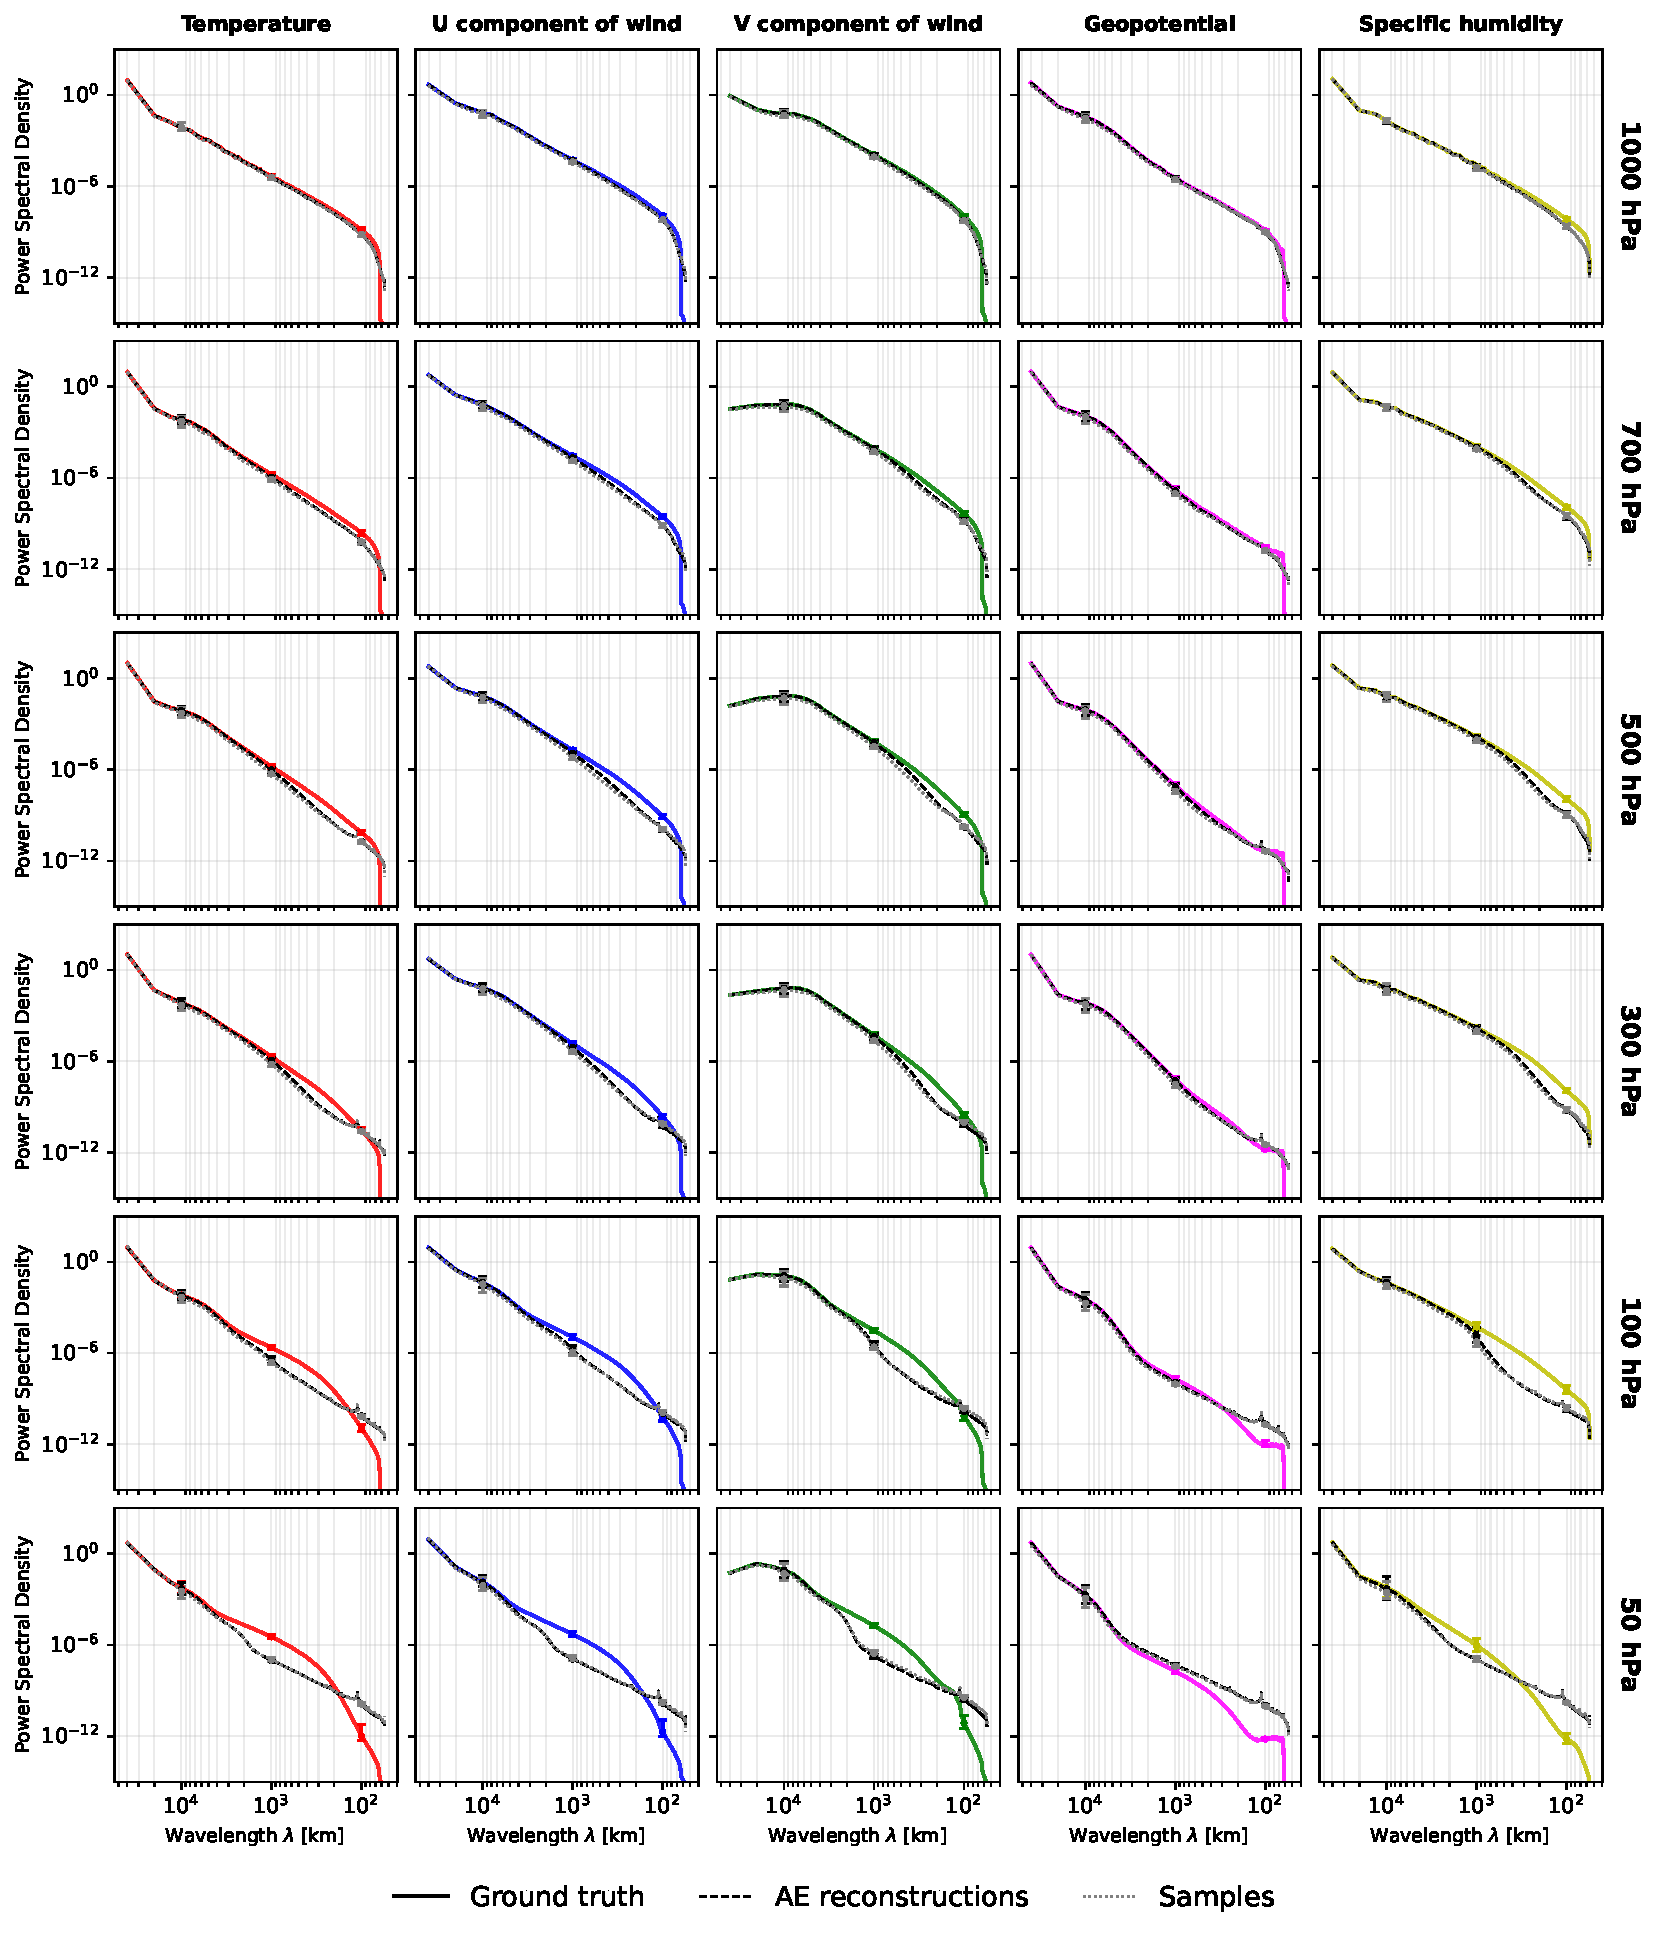
\includegraphics[width=\textwidth]{./chapters/appa/figures/power_spectra.pdf}
    \caption{Power spectral density across wavelengths for atmospheric fields at different pressure levels between January 2021 and December 2021. Lines show median values and error bars indicate the 5th to 95th percentiles. The close alignment between the curves demonstrates that both the autoencoder and the diffusion model preserve the energy distribution across most spatial scales. Deviations begin to appear at wavelengths around \qty{1000}{\kilo\meter}, which corresponds to roughly 40 pixels at the equator at our \qty{0.25}{\degree} resolution. These differences become more pronounced at smaller scales, suggesting that while large-scale atmospheric patterns are well-preserved, features spanning fewer than \qty{1000}{\kilo\meter} lose energy in the compression processes. Deviations become more pronounced at lower pressure levels, as the model prioritizes surface and low-altitude fields.}
\end{figure}

\begin{figure}[!h]
    \centering
    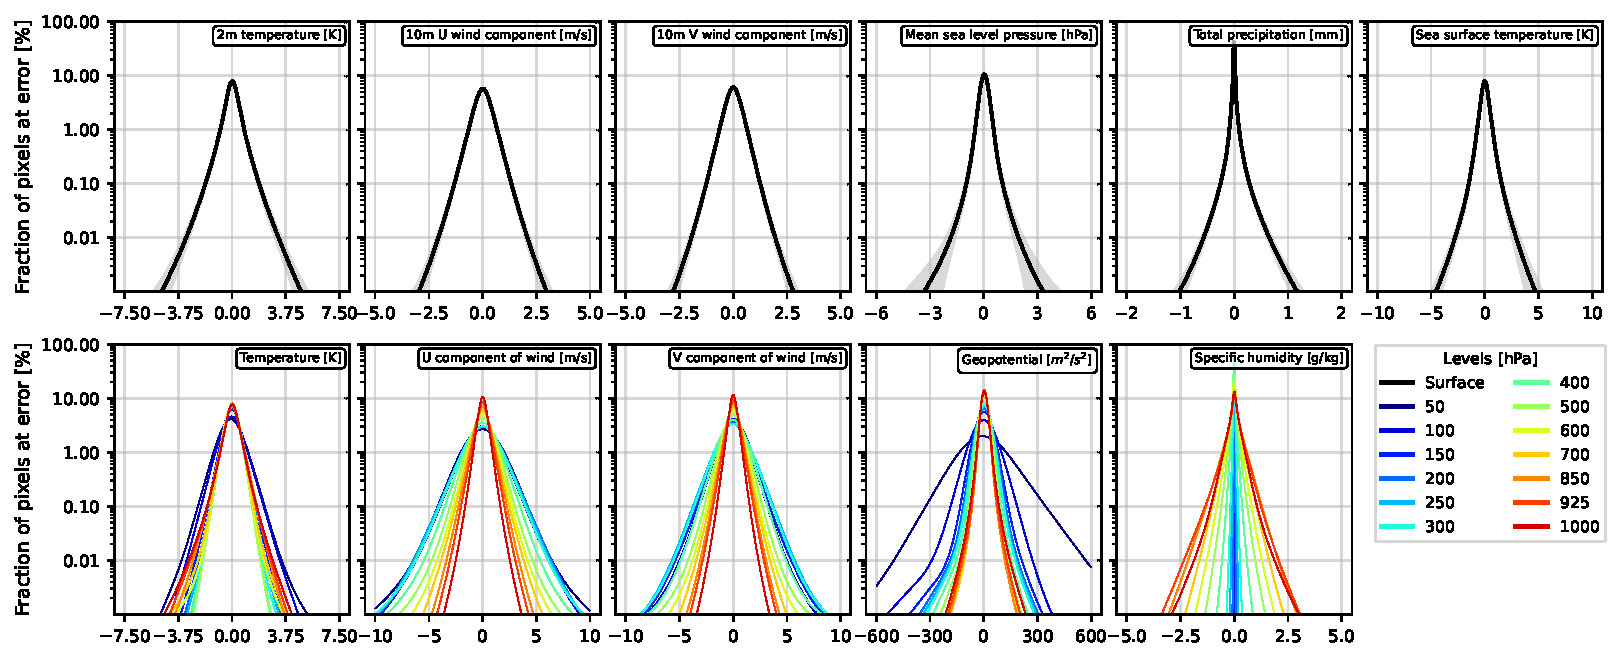
\includegraphics[width=\textwidth]{./chapters/appa/figures/ae_bells.pdf}
    \caption{Reconstruction bias distributions for surface fields across all grid points (top) and atmospheric fields across all pressure levels (bottom). The distributions centered around zero demonstrate unbiased and accurate reconstructions. For $\num{721} \times \num{1440} = \num{1038240}$ grid points, a \qty{0.01}{\percent} fraction on the y-axis corresponds to approximately 100 points, indicating that large biases are rare.}
    \label{fig:ae-bias}
\end{figure}

\begin{figure}[!h]
    \centering
    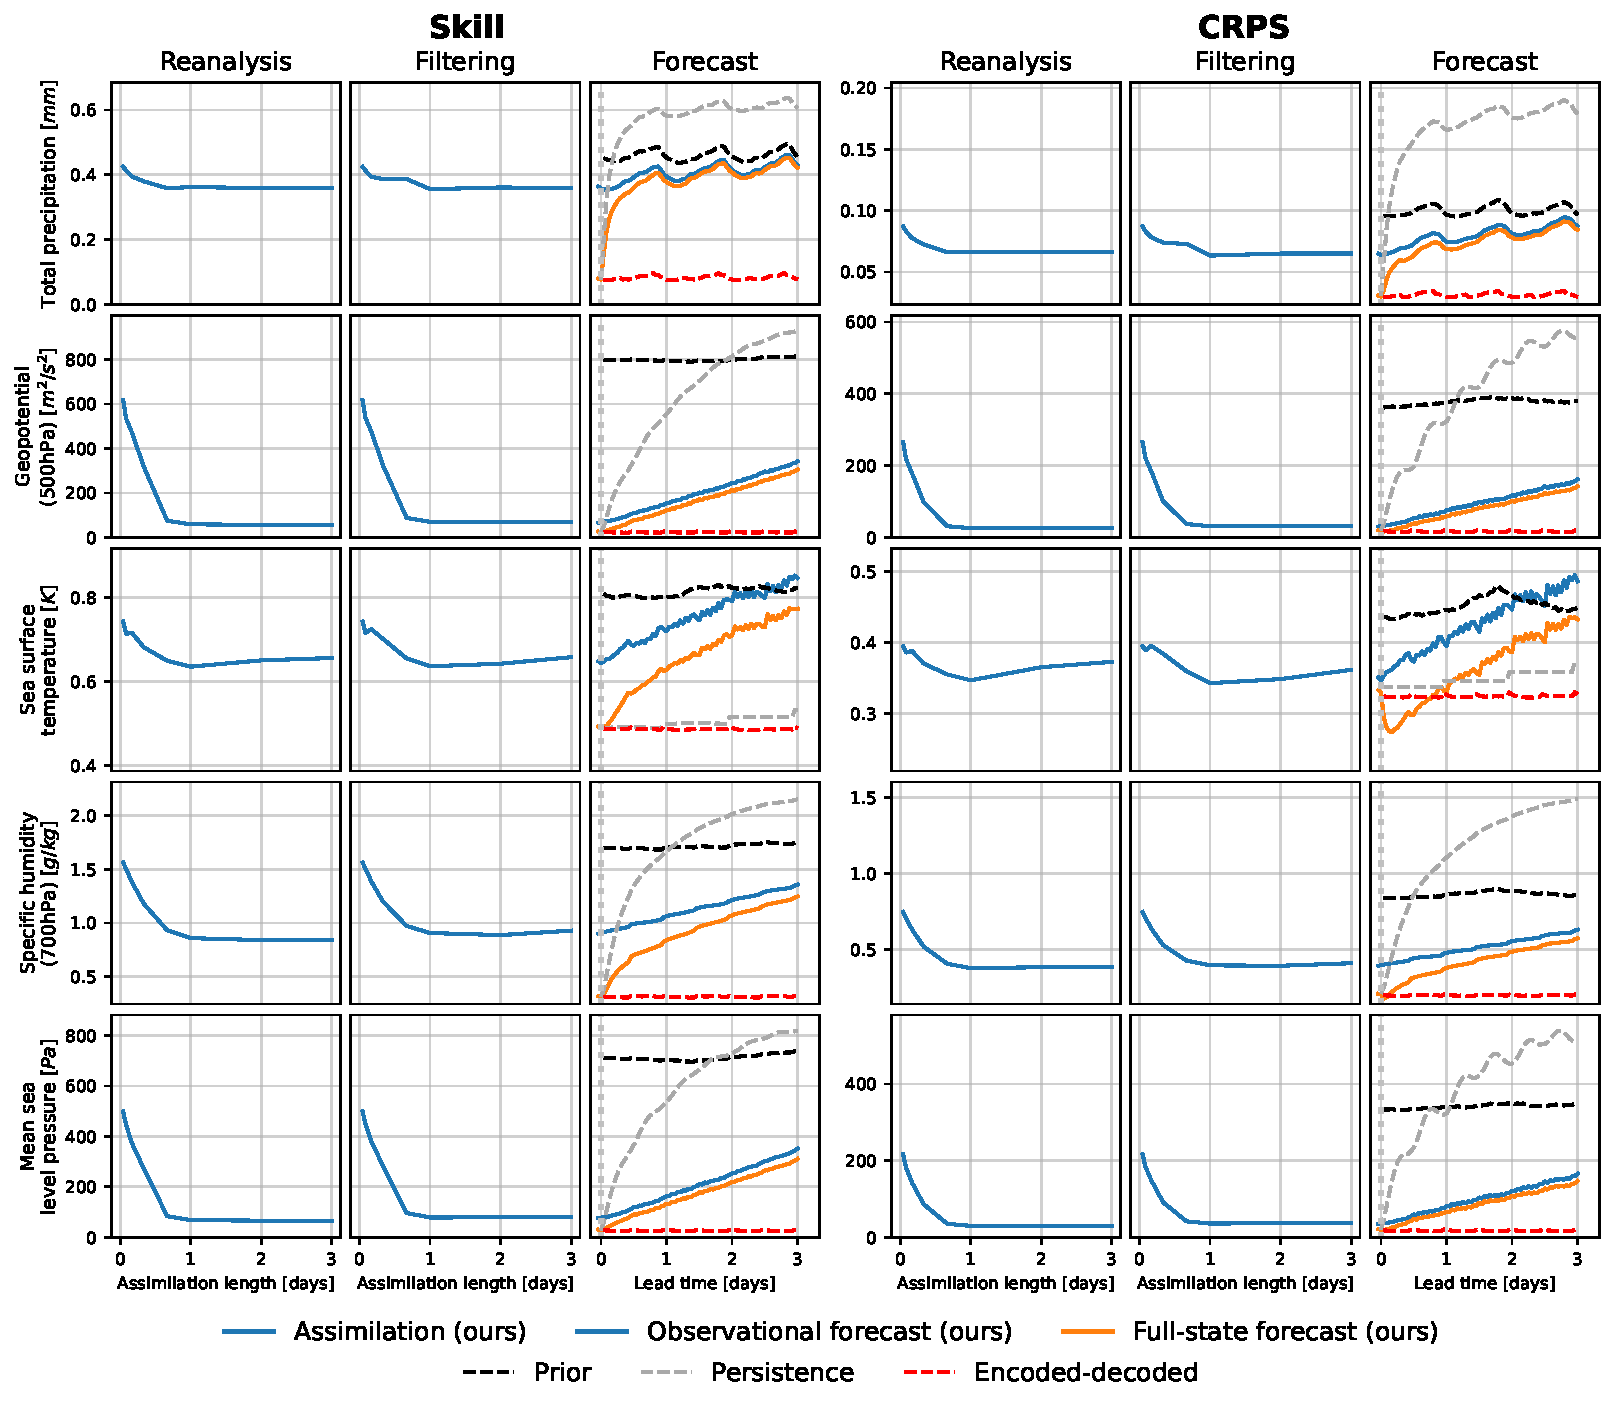
\includegraphics[width=\textwidth]{./chapters/appa/figures/skill_crps_appendix_2023.pdf}
    \caption{Skill and CRPS of other representative fields in assimilation tasks over January 2023. Reanalysis metrics are averaged over assimilation windows $x^{1:L}$, while filtering only considers the last assimilated state $x^L$. Both improve with longer assimilation windows, but eventually stagnate. Forecasts gradually lose skill over lead time. IFS~\cite{ecmwf2020ifs} and GraphDOP~\cite{alexe2024graphdop} are shown for reference.}
\end{figure}

\begin{figure}[!h]
    \centering
    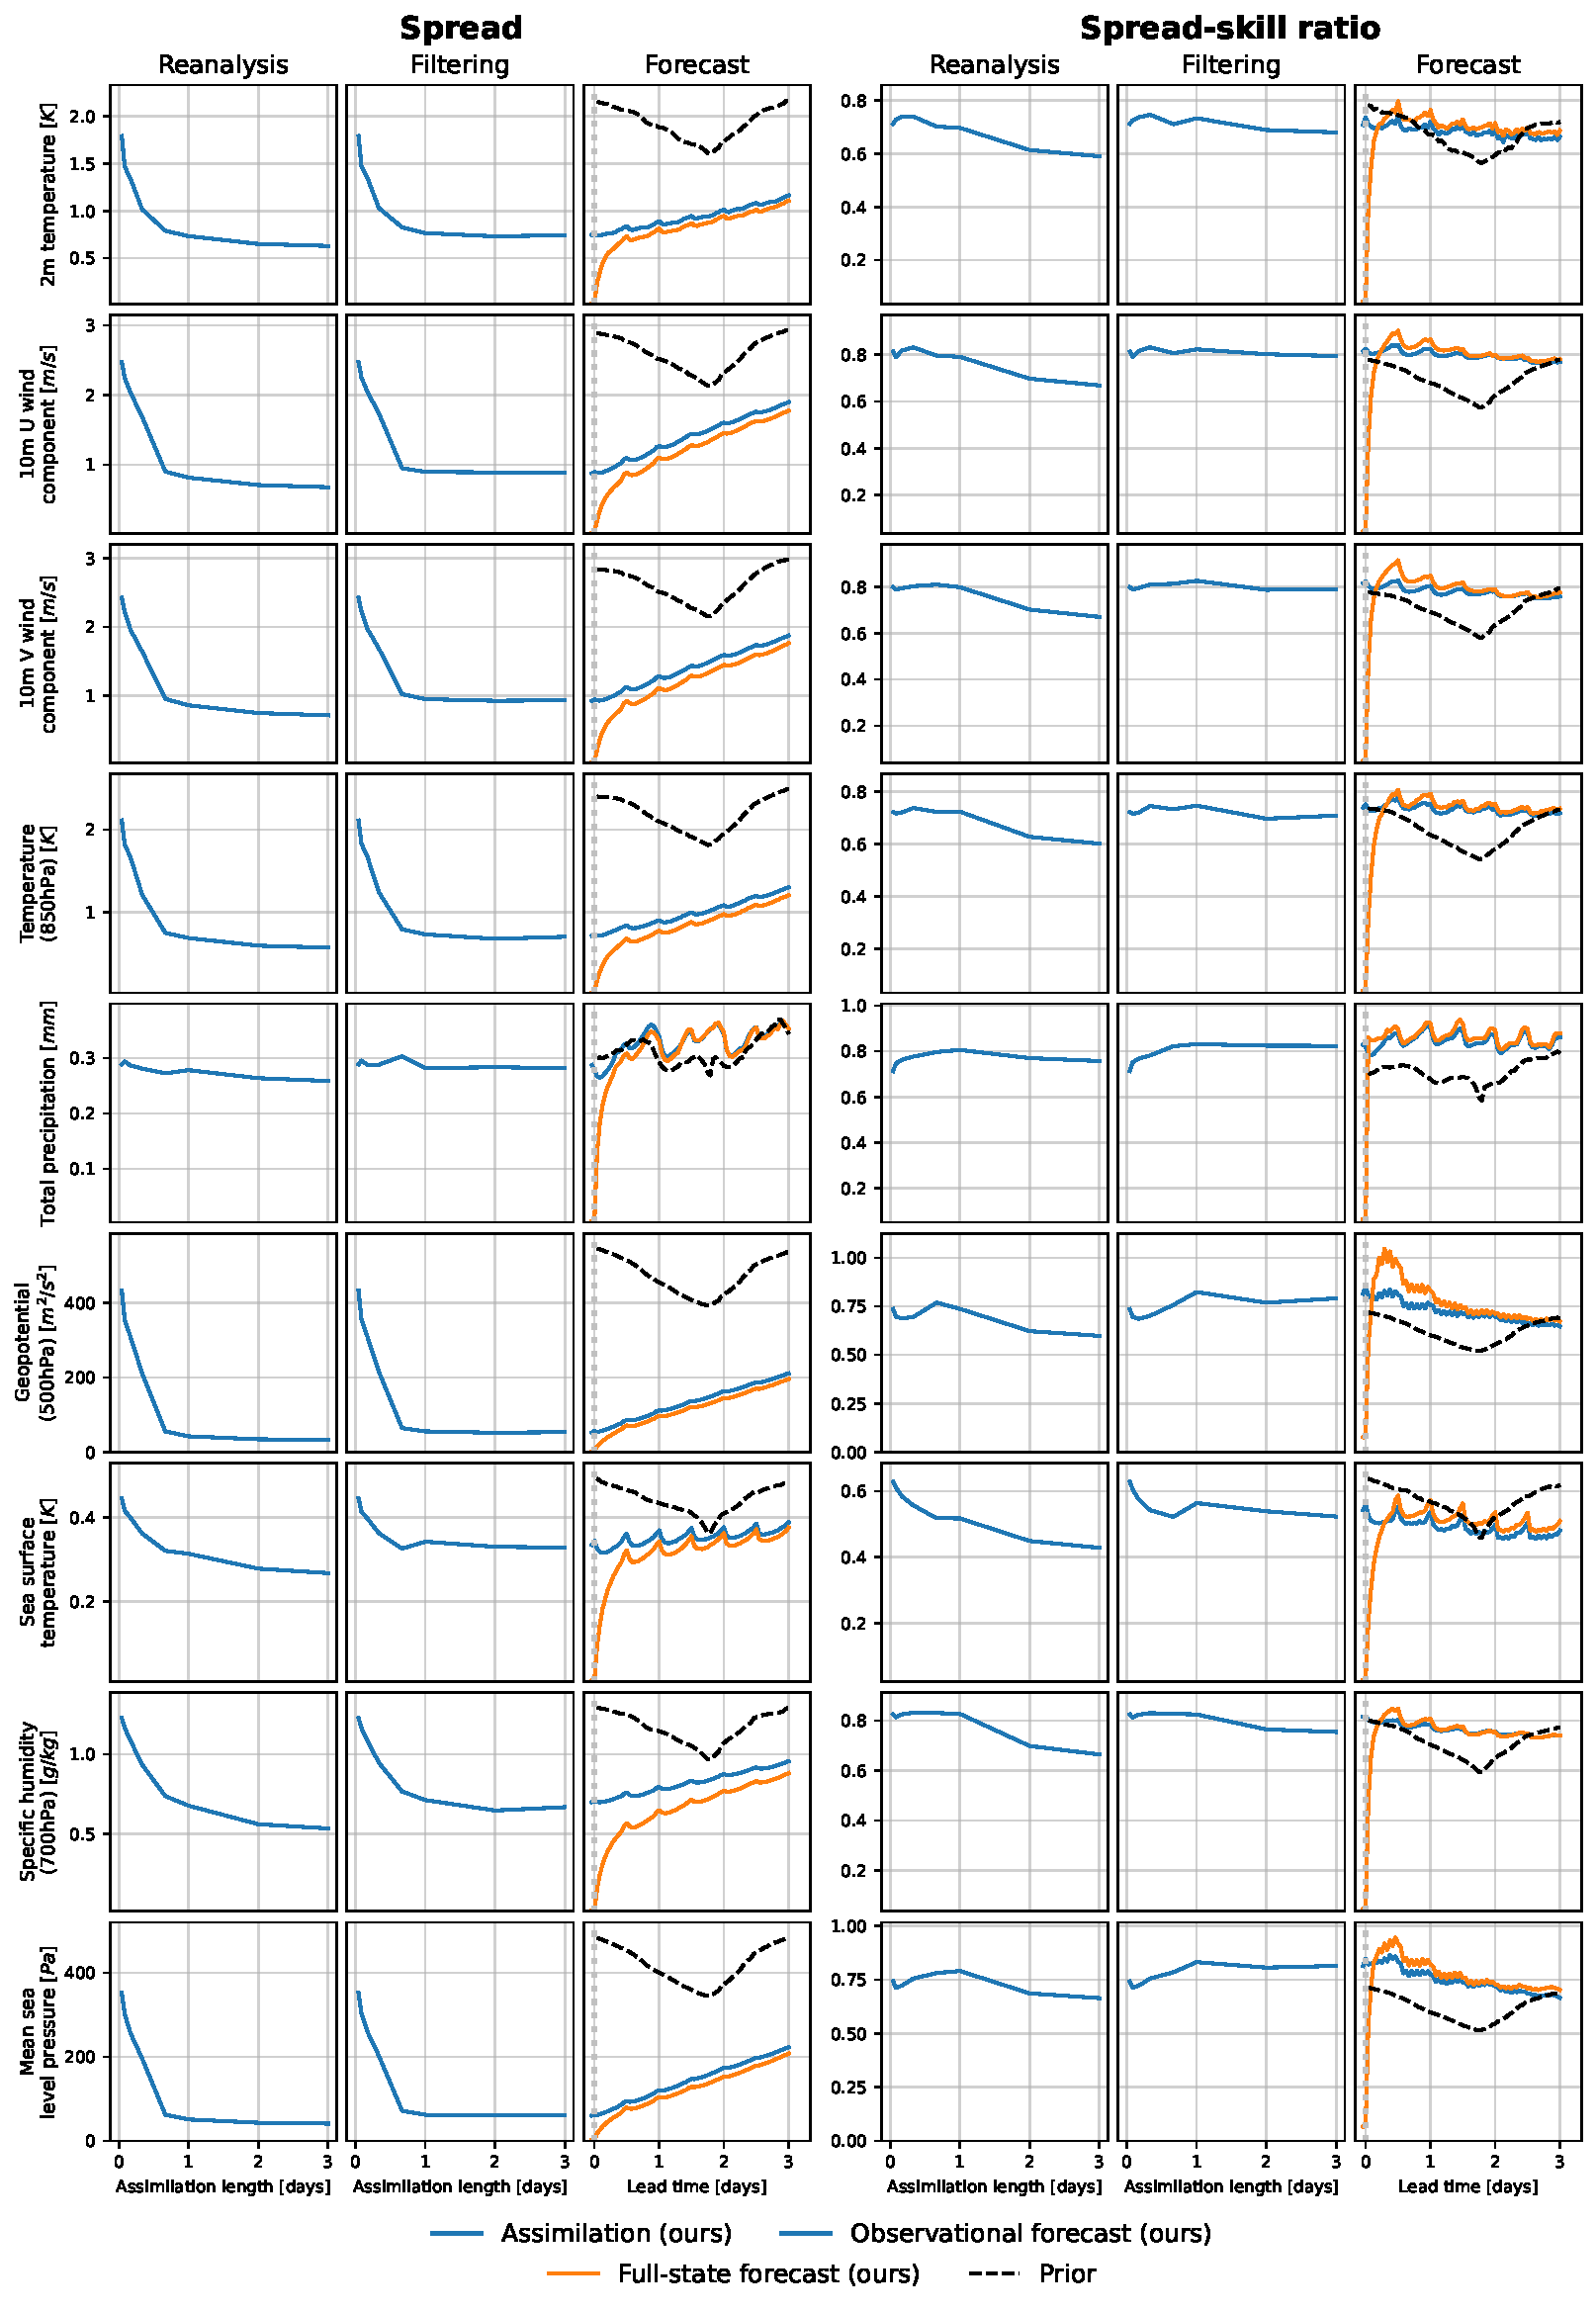
\includegraphics[width=\textwidth]{./chapters/appa/figures/spread_skill_ratio_2023.pdf}
    \caption{Spread and Spread-Skill ratio of representative fields in assimilation tasks over January 2023. Metrics are averaged over assimilation windows $x^{1:L}$, while filtering only considers the last assimilated state $x^L$. Ensemble spread (i.e. uncertainty) decreases with longer assimilation windows, while spread-skill ratios remain constant. A ratio below one indicates overconfidence.}
\end{figure}

\clearpage
\subsection{Physical consistency}

To further evaluate physical consistency, we examine whether our model preserves important physical relationships between variables. First, we analyze the consistency between two different estimators of altitude at given pressure levels. Using the geopotential $\Phi$, altitude can be derived as
\begin{equation}
    H = \frac{\Phi R_e}{g_{0}R_e-\Phi} \, ,
\end{equation}
where $R_e$ is Earth's radius and $g_{0}$ is the Earth gravitational acceleration at the surface. Alternatively, the equation below (which relies on the ideal gas law and hydrostatic equation) relates altitude to pressure and temperature as
\begin{equation}
    \log{\frac{p_0}{p_H}} = \frac{M g_0}{R}\int_0^H \frac{1}{T_h} \partial{h} \, ,
\end{equation}
where $R$ is the universal gas constant, $M$ is an approximation of the atmosphere's molar mass, $p_h, T_h$ are pressure and temperature at height $h$, and $p_0$, $T_0$ are the theoretical pressure and temperature at sea level. This integral can be approximated to extract $H$ using several assumptions about the temperature profile. When comparing these two estimators, Figure~\ref{fig:physical-consistency} shows that our generated samples maintain the same systematic differences $\Delta H$ as seen in ground-truth data. This remarkable consistency indicates that our model successfully preserves this physical relationships between temperature, pressure, and geopotential, allowing altitude to be estimated through two independent methods with nearly identical accuracy to the original ERA5 data.

Second, we examine the geostrophic balance
\begin{align}
    \frac{\partial \Phi}{\partial x} & = \frac{4 \pi \Omega R_e}{N_x} \sin{\phi} \cos{\phi} u_g\\
    \frac{\partial \Phi}{\partial y} & = -\frac{2 \pi \Omega R_e}{N_y} \sin{\phi} v_g
\end{align}
which is the theoretical equilibrium between pressure gradient forces and Coriolis forces that governs large-scale atmospheric motion. In the above system, $\phi$ is the latitude, $N_x$ and $N_y$ are the number of pixels along longitude and latitude, $\Omega$ is the magnitude of the Earth's angular velocity, and $u_g$ and $v_g$ denote the eostrophic components of the wind. In this balance, in the absence of vertical motion, friction, and isobaric curvature, wind direction should be perpendicular to geopotential gradients, with wind speed proportional to gradient magnitude. This relationship can be expressed by comparing two quantities: (1) the angle $\theta$ between wind and geopotential gradients, which should approach \qty{90}{\degree} in geostrophic conditions, and (2) the correlation between wind speed magnitude and geopotential gradient magnitude, which should approach 1 in perfect geostrophic balance. Figure~\ref{fig:physical-consistency} shows that our generated samples accurately reproduce both aspects of this relationship. At \qty{500}{\hecto\pascal}, the approximate level of non-divergence with minimal surface friction effects, both ERA5 data and our generated samples show angles concentrated around \qty{90}{\degree}. Near the surface at \qty{1000}{\hecto\pascal}, where additional forces become significant, both datasets show a systematic deviation in angle. Similarly, the correlation between wind speed and geopotential gradient magnitudes in our samples closely matches the patterns observed in ERA5 data, exhibiting imperfect correlation only at lower pressure levels (explained by the level-weighted training) and following the same decreasing trend as pressure increases toward the surface, where ageostrophic components become more prominent.

These results demonstrate that our latent diffusion model not only preserves the statistical properties of atmospheric fields but also maintains important physical relationships between variables producing trajectories that are physically consistent and realistic. While these analyses confirm strong spatial consistency and physical fidelity, future work should extend our evaluation to more thoroughly quantify the temporal consistency of generated trajectories.

\begin{figure}[!h]
    \centering
    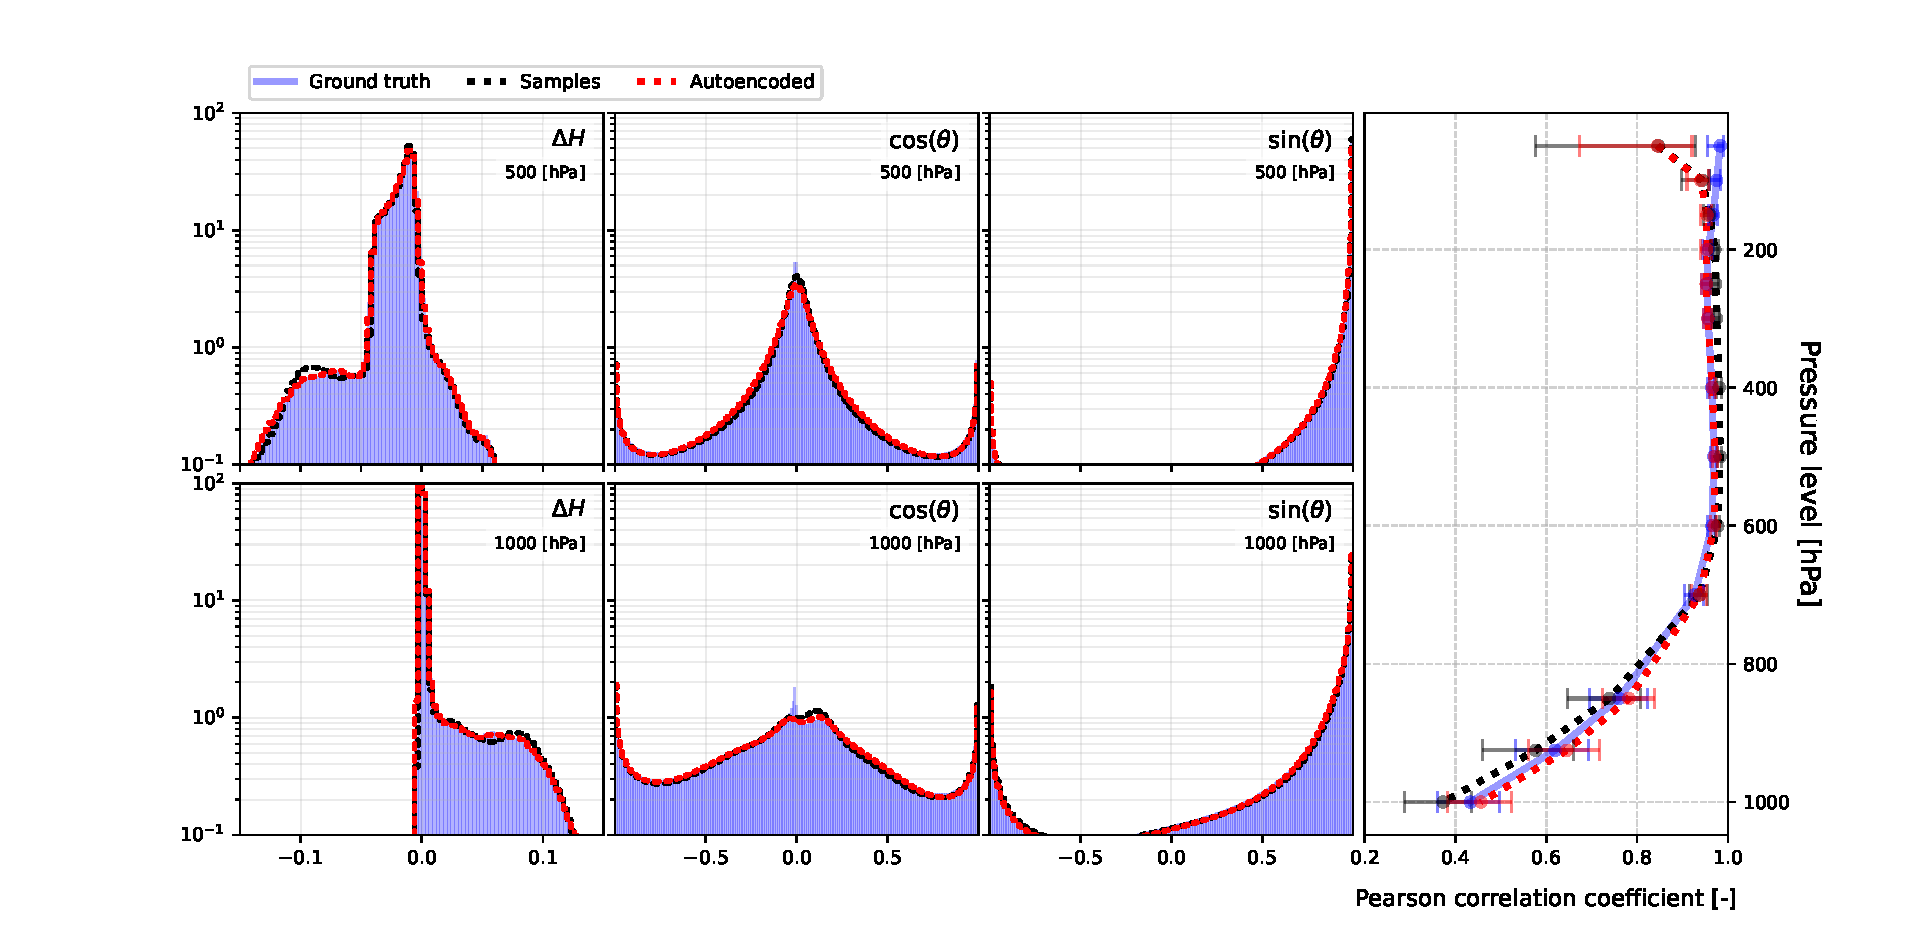
\includegraphics[width=\textwidth]{./chapters/appa/figures/physical_consistency.pdf}
    \caption{Physical consistency analysis of generated atmospheric states.
    \textbf{(top)} Analysis of altitude consistency at \qty{500}{\hecto\pascal} showing the difference $\Delta H$ between two independent altitude estimators, and geostrophic balance assessment through the cosine and sine of the angle $\theta$ between wind direction and geopotential gradients, demonstrating angles concentrated around \qty{90}{\degree}.
    \textbf{(bottom)} Same metrics at \qty{1000}{\hecto\pascal} demonstrating the presence of a significant ageostrophic component near the surface.
    \textbf{(right)} Correlation coefficient between wind magnitude and geopotential gradient magnitude across pressure levels, showing strong correlation at upper levels (near 1) with a consistent decrease toward the surface in both ERA5 data (blue) and generated samples (black dots), confirming Appa's ability to capture complex physical relationships.}
    \label{fig:physical-consistency}
\end{figure}

\clearpage
\subsection{Qualitative snapshots}

In Figures \ref{fig:gallery_t2m} to \ref{fig:gallery_z850}, we illustrate trajectories generated through reanalysis over a window of $L=72$ hours or through forecasting, for six representative fields. The second row of each gallery shows the observed pixels, if any. Surface fields and atmospheric fields have different observation masks (ground station network vs. satellite orbital).

\begin{figure}[!h]
    \centering
    \includegraphics[width=\textwidth]{./chapters/appa/compressed/gallery/reanalysis/2m_temperature.pdf}
    \includegraphics[width=\textwidth]{./chapters/appa/compressed/gallery/forecasting/2m_temperature.pdf}
    \caption{Sampled trajectories for surface temperature assimilation. Reanalysis (top) and observational forecasting (bottom) over a window of 72 hours.}
    \label{fig:gallery_t2m}
\end{figure}

\begin{figure}
    \centering
    \includegraphics[width=\textwidth]{./chapters/appa/compressed/gallery/reanalysis/10m_u_component_of_wind.pdf}
    \includegraphics[width=\textwidth]{./chapters/appa/compressed/gallery/forecasting/10m_u_component_of_wind.pdf}
    \caption{Sampled trajectories for surface zonal wind speed assimilation. Reanalysis (top) and observational forecasting (bottom) over a window of 72 hours.}
    \label{fig:gallery_10u}
\end{figure}

\begin{figure}
    \centering
    \includegraphics[width=\textwidth]{./chapters/appa/compressed/gallery/reanalysis/10m_v_component_of_wind.pdf}
    \includegraphics[width=\textwidth]{./chapters/appa/compressed/gallery/forecasting/10m_v_component_of_wind.pdf}
    \caption{Sampled trajectories for surface meridional wind speed assimilation. Reanalysis (top) and observational forecasting (bottom) over a window of 72 hours.}
    \label{fig:gallery_10v}
\end{figure}

\begin{figure}
    \centering
    \includegraphics[width=\textwidth]{./chapters/appa/compressed/gallery/reanalysis/total_precipitation.pdf}
    \includegraphics[width=\textwidth]{./chapters/appa/compressed/gallery/forecasting/total_precipitation.pdf}
    \caption{Sampled trajectories for total precipitation assimilation. Reanalysis (top) and observational forecasting (bottom) over a window of 72 hours.}
    \label{fig:gallery_tp}
\end{figure}

\begin{figure}
    \centering
    \includegraphics[width=\textwidth]{./chapters/appa/compressed/gallery/reanalysis/specific_humidity_700hPa.pdf}
    \includegraphics[width=\textwidth]{./chapters/appa/compressed/gallery/forecasting/specific_humidity_700hPa.pdf}
    \caption{Sampled trajectories for specific humidity assimilation at \qty{700}{\hecto\pascal}. Reanalysis (top) and observational forecasting (bottom) over a window of 72 hours.}
    \label{fig:gallery_q700}
\end{figure}

\begin{figure}
    \centering
    \includegraphics[width=\textwidth]{./chapters/appa/compressed/gallery/reanalysis/geopotential_850hPa.pdf}
    \includegraphics[width=\textwidth]{./chapters/appa/compressed/gallery/forecasting/geopotential_850hPa.pdf}
    \caption{Sampled trajectories for geopotential assimilation at \qty{850}{\hecto\pascal}. Reanalysis (top) and observational forecasting (bottom) over a window of 72 hours.}
    \label{fig:gallery_z850}
\end{figure}

\end{subappendices}
